% https://tex.stackexchange.com/a/50906/173708

\documentclass[border=10pt]{standalone}
\usepackage{tikz}
\usetikzlibrary{trees}

\begin{document}

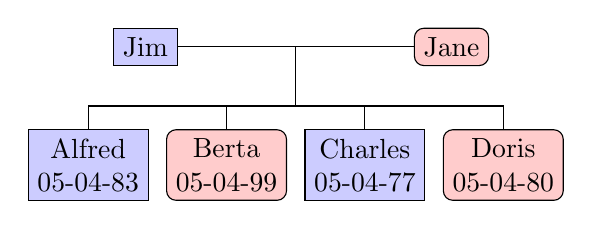
\begin{tikzpicture}[
	man/.style={rectangle, 
				draw, 
				fill=blue!20, 
				align=center},
	woman/.style={rectangle, 
					draw, 
					fill=red!20,
					rounded corners=.8ex, 
					align=center},
	grandchild/.style={grow=down, 
						xshift=1em, 
						anchor=west,
						edge from parent path={(\tikzparentnode.south) |- (\tikzchildnode.west)}},
	first/.style={level distance=6ex},
	second/.style={level distance=12ex},
	third/.style={level distance=18ex},
	level 1/.style={sibling distance=5em}]
	% Parents
	\coordinate
	child[grow=left] {node[man,anchor=east]{Jim}}
	child[grow=right] {node[woman,anchor=west]{Jane}}
	child[grow=down,level distance=0ex]
	[edge from parent fork down]
	% Children and grandchildren
	child{node[man] {Alfred \\ 05-04-83}}
	child{node[woman] {Berta \\ 05-04-99}}
	child {node[man] {Charles \\ 05-04-77}}
	child {node[woman]{Doris \\ 05-04-80}};        
\end{tikzpicture}

\end{document}